\subsection{Schiefe Mercatorprojektion}
\label{sec:schiefmerc}
Bei der schiefen Mercatorprojektion kann die zentrale Linie jede Linie zwischen zwei Punkten sein und nicht wie bei der Mercatorprojektion nur ein Breitengrad oder der transversen Mercatorprojektion nur ein Längengrad.\\
\begin{figure}[hbtp]
\centering
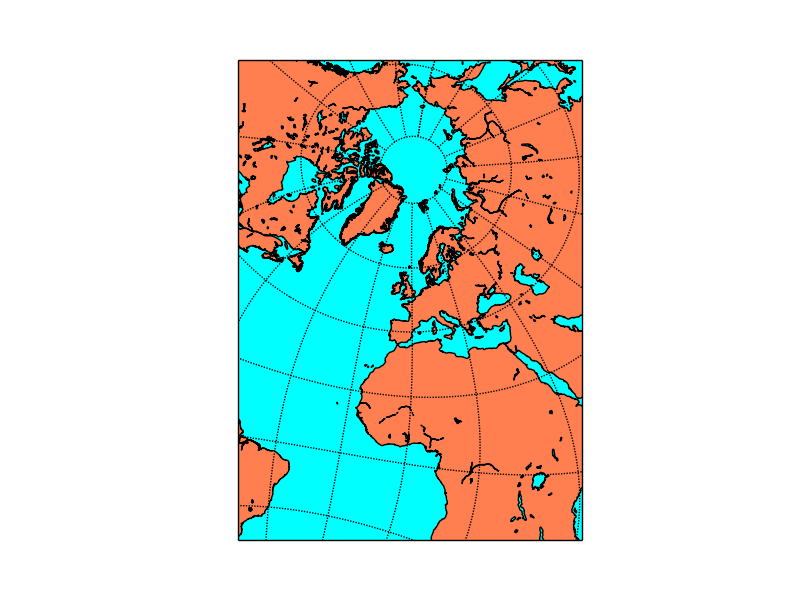
\includegraphics[scale=0.5,origin=c]{/Users/student/seminar/Kartendarstellungen/seminar/omerc.png}
\caption{Schiefe Mercatorprojektion}
\end{figure}
\newpage 
%\begin{center}
%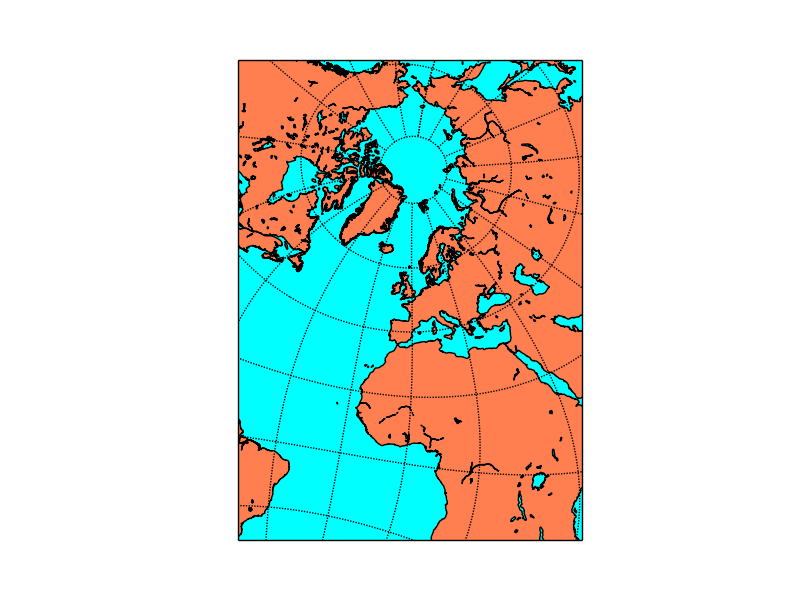
\includegraphics[origin=c]{/Users/student/seminar/Kartendarstellungen/seminar/omerc} \newpage 
%\end{center}